\documentclass[9pt]{beamer}

\usetheme{TUDo}

% Sprachumgebung
\usepackage[ngerman]{babel}


% Encoding je nach Compiler
\ifluatex
\usepackage[utf8]{luainputenc}
\else
\usepackage[utf8]{inputenc}
\usepackage[T1]{fontenc}
\fi


% Mathematik
\usepackage{amsmath}
\usepackage{amsfonts}
\usepackage{amssymb}
\usepackage{cancel}

%Links
\usepackage[]{hyperref}

%%%%%%%%%%%%%%%%%%%%%%%%%%%%%%%%%%%%%%%%%%%%%%%%%%%%%%%%%%%%%%%%%%%%%%%%%%%%%%%%
%%%%%-------------Hier Titel/Autor/Grafik/Lehrstuhl eintragen--------------%%%%%
%%%%%%%%%%%%%%%%%%%%%%%%%%%%%%%%%%%%%%%%%%%%%%%%%%%%%%%%%%%%%%%%%%%%%%%%%%%%%%%%

%Titel:
\title{Das neue \LaTeX-Beamer-Theme der \mbox{TU Dortmund}}
%Autor
\author{Maximilian Nöthe}
%Lehrstuhl/Fakultät
\institute[Lehrstuhl\\Fakultät]{Names des Lehrstuhls /\par\smallskip\smallskip Name der Fakultät}
%Titelgrafik 
\titlegraphic{TUDo-Title-Pic-2.jpg}


\begin{document}

\begin{frame}
\setcounter{framenumber}{0}
    \titlepage
\end{frame}

\begin{frame}
    \frametitle{Wichtige Hinweise}
    Zu diesem Theme
    \begin{itemize}
        \item Die .sty-Files müssen im gleichen Verzeichnis wie die .tex liegen
        \item Ebenso das TU-Logo und eventuelle andere Bilder 
    \end{itemize}
    Allgemein zu Beamer und Latex:
    \begin{itemize}
        \item Latex-Beamer Dokumetation:\\
            \url{http://texdoc.net/texmf-dist/doc/latex/beamer/doc/beameruserguide.pdf}
        \item Modern Packages for Latex, sehr lesenswert:
            \url{http://philippleser.de/physics/latex}
    \end{itemize}
\end{frame}

\begin{frame}
    \frametitle{Einführung}
    \tableofcontents[pausesections]
\end{frame}

\section{Blindtext}
\begin{frame}
	\frametitle{Hier steht eine lange, zweizeilige Headline
		\newline gefolgt von einem Blindtext}
Dieser Text dient nur zur Veranschaulichung des Textsatzes. Niemand sollte jemals, aus keinem noch so gutem Grund, so viel Text auf eine Folie packen.

Dies ist ein Blindtext. Dieser Text ist nicht dafür vorgesehen, den Betrachter in die Welt der Dunkelheit zu führen, sondern dafür, einfach etwas Leeres mit etwas Inhaltlosem zu füllen.

Dies ist ein Blindtext. Dieser Text ist nicht dafür vorgesehen, den Betrachter in die Welt der Dunkelheit zu führen, sondern dafür, einfach etwas Leeres mit etwas Inhaltlosem zu füllen.

Dies ist ein Blindtext. Dieser Text ist nicht dafür vorgesehen, den Betrachter in die Welt der Dunkelheit zu führen, sondern dafür, einfach etwas Leeres mit etwas Inhaltlosem zu füllen.

\end{frame}

\section{Formelsatz}
\begin{frame}
	\frametitle{Formelsatz}
	\begin{block}{Mathematischer Formelsatz ist eine Spezialität von \LaTeX}
		\[
		u(x,t)= 8 \frac{k_{1}^{2}e^{\alpha_{1}} + k_{2}^{2}e^{\alpha_{2}} + (k_{1}-k_{2})^{2}e^{(\alpha_{1}+ \alpha_{2})} \left[2 + \frac{1}{(k_{1} + k_{2})^{2}} ( k_{1}^{2}e^{\alpha_{1}} + k_{2}^{2}e^{\alpha_{2}}) \right]}{\left[1+e^{\alpha_{1}} + e^{\alpha_{2}} + \left(\frac{k_{1} - k_{2}}{k_{1}+k_{2}} \right)^{2} e^{\alpha_{1}+ \alpha_{2}} \right]^{2}}
		\]
		\[
			t-t_{0}=\sqrt{\frac{l}{g}}\int_{0}^{\varphi}{\frac{\mathrm{d}\psi}{\sqrt{1-k^{2}\sin^{2} {\psi}}}} = \sqrt{\frac{l}{g}} F(k,\varphi)
		\]
		\[
			\frac{\binom{\sqrt[15]{\pi}}{\infty}}{\pm G - x_{62}^{34}} = \varliminf \sum \frac{\cos \mho}{\sin \eth}
		\]
	\end{block}
\end{frame}

\begin{frame}
	\begin{columns}
		\begin{column}{0.49\textwidth}
			\begin{exampleblock}{Brüche}
				\[\frac{2+dc}{9}\]
			\end{exampleblock}
			\begin{exampleblock}{Wurzeln}
				\[
					\sqrt{x}
					\quad\text{bzw.}\quad
					\sqrt[n]{x}
				\]
			\end{exampleblock}
			\begin{exampleblock}{Indizes \& Hochstellungen}
				\[a_{b_c} \quad\text{und}\quad a^{2^3}\]
			\end{exampleblock}
			\begin{exampleblock}{Summen}
				\[\sum\limits_{i=1}^n i = \frac{n(n+1)}{2}\]
			\end{exampleblock}
		\end{column}
		\begin{column}{0.49\textwidth}
			\begin{exampleblock}{Produkte}
				\[\prod\limits_{i=1}^{n+1}i = 1\cdot 2\cdot\ldots\cdot n\cdot (n+1)\]
			\end{exampleblock}
			\begin{exampleblock}{Integrale}
				\[
					\int_0^3 x^2\,\mathrm{d}x = 9
					\quad\text{oder}\quad
					\int\limits_0^3 x^2 \,\mathrm{d}x = 9
				\]
			\end{exampleblock}
			\begin{exampleblock}{Doppel- und Mehrfachintegrale}
				\[
					\iint_a^b
					\quad\text{oder}\quad
					\idotsint_a^b
				\]
			\end{exampleblock}
		\end{column}
	\end{columns}
\end{frame}

\begin{frame}
	\begin{columns}
		\begin{column}{0.49\textwidth}
			\begin{exampleblock}{Limes}
				\[\lim_{n \to \infty}\frac{1}{n}=0\]
			\end{exampleblock}
			\begin{exampleblock}{Sonderzeichen}
                \begin{align*}
                    \leq \geq \ll \gg \cdot \times\\
                    \Rightarrow \rightarrow \propto \approx \in \not\in
                \end{align*}
			\end{exampleblock}
			\begin{exampleblock}{Referenzieren}
				\begin{equation}
					r_1^2 = x^2 + y^2
					\label{eq:formel}
				\end{equation}
				Referenzen als Formelnummer \ref{eq:formel} oder
				als	Formelnummer mit Klammer \eqref{eq:formel}.
				% \pageref{eq:formel}.
			\end{exampleblock}
		\end{column}
		\begin{column}{0.49\textwidth}
			\begin{exampleblock}{Matrizen}
				\[
					\left(
						\begin{array}{ccc}
							a_{11} & \cdots & a_{1n} \\
							\vdots & \ddots & \vdots \\
							a_{m1} & \cdots & a_{mn}
						\end{array}
					\right)
				\]
				\[
					\begin{pmatrix}
						\kappa_{11} & \cdots & \kappa_{1n} \\
						\vdots      & \ddots & \vdots      \\
						\kappa_{m1} & \cdots & \kappa_{mn}
					\end{pmatrix}
				\]
			\end{exampleblock}
			\begin{exampleblock}{Durchstreichungen}
				\[
					\frac{13}{39} = \cancel{{\frac{13}{13}}} \cdot \frac{1}{3}
					\quad\text{oder}\quad
					\frac{13}{39} = \frac{\cancel{13} \cdot 1}{\cancel{13} \cdot 3}
				\]
			\end{exampleblock}
		\end{column}
	\end{columns}
\end{frame}

\section{Das Design}
\subsection{Farben}
\begin{frame}
    \frametitle{Eine TU-Farbpalette: Herbstlich (warm)}
    Farben können über die üblichen \LaTeX-Pakete wie \emph{xcolor} definiert und mit Hilfe der Beamer Befehle gesetzt werden.
    Siehe hierzu den vorn verlinkten \emph{Beamer-Users-Guide}. Es wird jedoch empfohlen die TU-Farbpalette zu nutzen:
    \begin{itemize}
        \item \textcolor{TUgreen}{Dies istTUgreen}
            \begin{itemize}
                \item \textcolor{TUlightgreen}{Dies ist TUlightgreen}
                \item \textcolor{TUdarkgreen}{Dies ist TUdarkgreen}
                \item \textcolor{TUolive}{Dies ist TUolive}
            \end{itemize}
        \item \textcolor{TUyellow}{Dies ist TUyellow}
        \item \textcolor{TUcitron}{Dies ist TUcitron}
        \item \textcolor{TUlime}{Dies ist TUlime}
        \item \textcolor{TUorange}{Dies ist TUorange}
    \end{itemize}
\end{frame}

\subsection{Blöcke}
\begin{frame}
    \frametitle{Verschiedene Block-Typen}
    \begin{block}{block}
        \begin{itemize}
            \item Standardblock
            \item für normalen, strukturierten Text
        \end{itemize}
    \end{block}
    \begin{alertblock}{alertblock}
        \begin{itemize}
            \item Block in auffallender Farbe
			\item zur Hervorhebung
        \end{itemize}
    \end{alertblock}
    \begin{exampleblock}{exampleblock}
        \begin{itemize}
            \item Ein anderer Block
			\item für Beispiele
        \end{itemize}
    \end{exampleblock}
\end{frame}

\section{Beispiel-Folien}
\subsection{Zweispaltige Layouts}
\begin{frame}
    \frametitle{Zwei Spalten für Text}
    \begin{columns}[T]
        \begin{column}{0.49\textwidth}
            \begin{itemize}[<+->] % Die ganze Liste erscheint der Reihe nach
                \item Erster  Eintrag
                \item Zweiter Eintrag
			    \item Dritter Eintrag
		    \end{itemize}
        \end{column}
        \begin{column}{0.49\textwidth}
		    \begin{enumerate}
			    \item<1-> Dieser Eintrag erscheint direkt
                \item<2>  Dieser Eintrag erscheint nur nach dem zweiten Klick
                \item<1-3> Dieser Punkt erscheint von 1-3
          \end{enumerate}
          \begin{itemize}[<+->]
              \item Erster  Punkt
              \item Zweiter Punkt
              \item Dritter Punkt
          \end{itemize}
        \end{column}
    \end{columns}
\end{frame}

\begin{frame}
    \frametitle{Je eine Spalte für Text/Bild}
    % Für Bilder Argument T benutzen:
    \begin{columns}[T]
        \begin{column}{0.49\textwidth}
            \begin{itemize}%[<+->] Kommentar entfernen falls jeder Punkt einzeln erscheinen soll
            \item Erster Eintrag
            \item Zweiter längerer Eintrag\\
							ausgedehnt auf drei Zeilen\\
							und manuellem Umbruch
            \item Dritter Eintrag
            \item Vierter Eintrag
			\item Fünfter Eintrag mit etwas mehr Text und automatischem Umbruch
            \item Sechster Eintrag
			\item[$\,\blacktriangleright$] Siebter Eintrag, anderes Symbol
        \end{itemize}
        \end{column}
        \begin{column}{0.49\textwidth}
            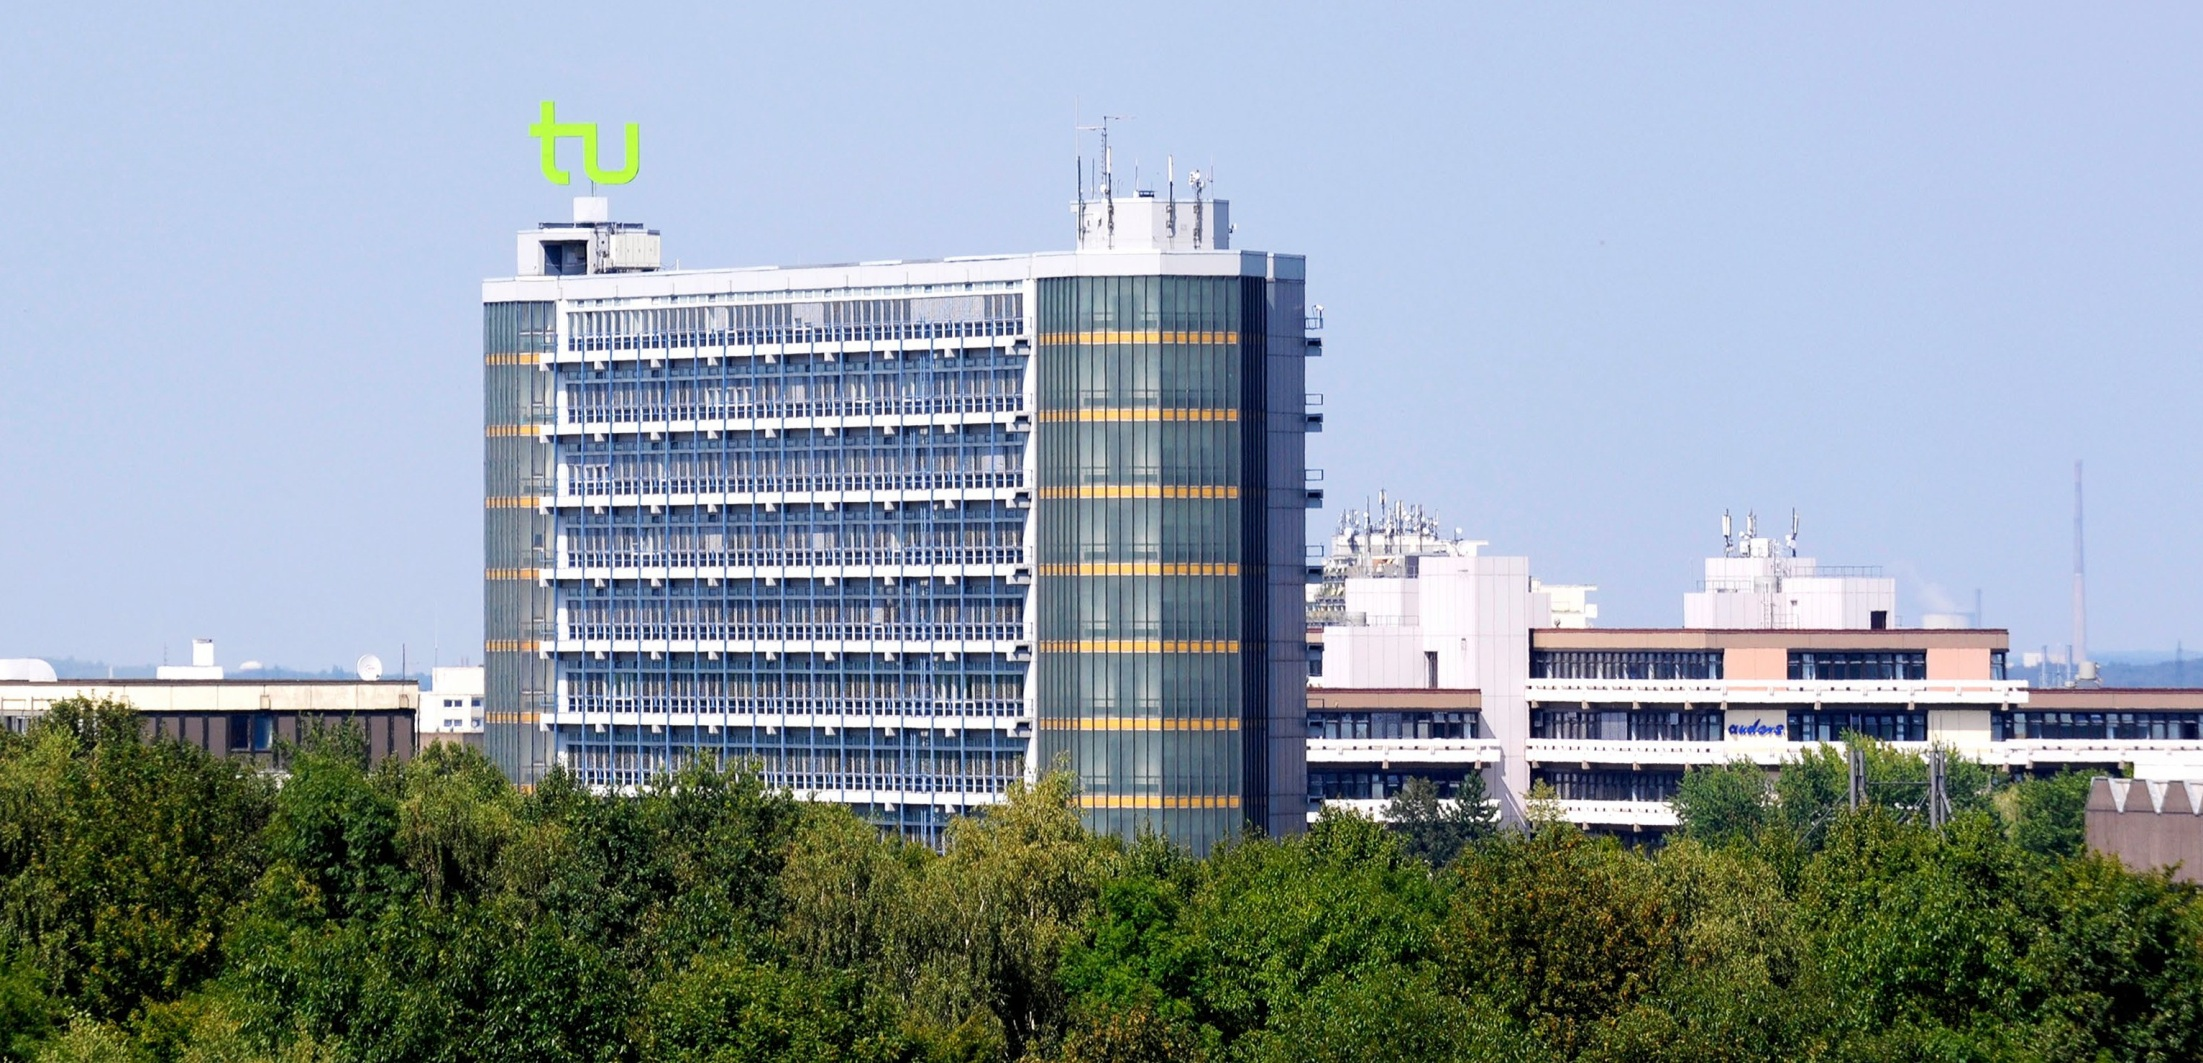
\includegraphics[width=\textwidth]{./TUDo-Title-Pic-1.jpg}
            \vspace{5pt}
			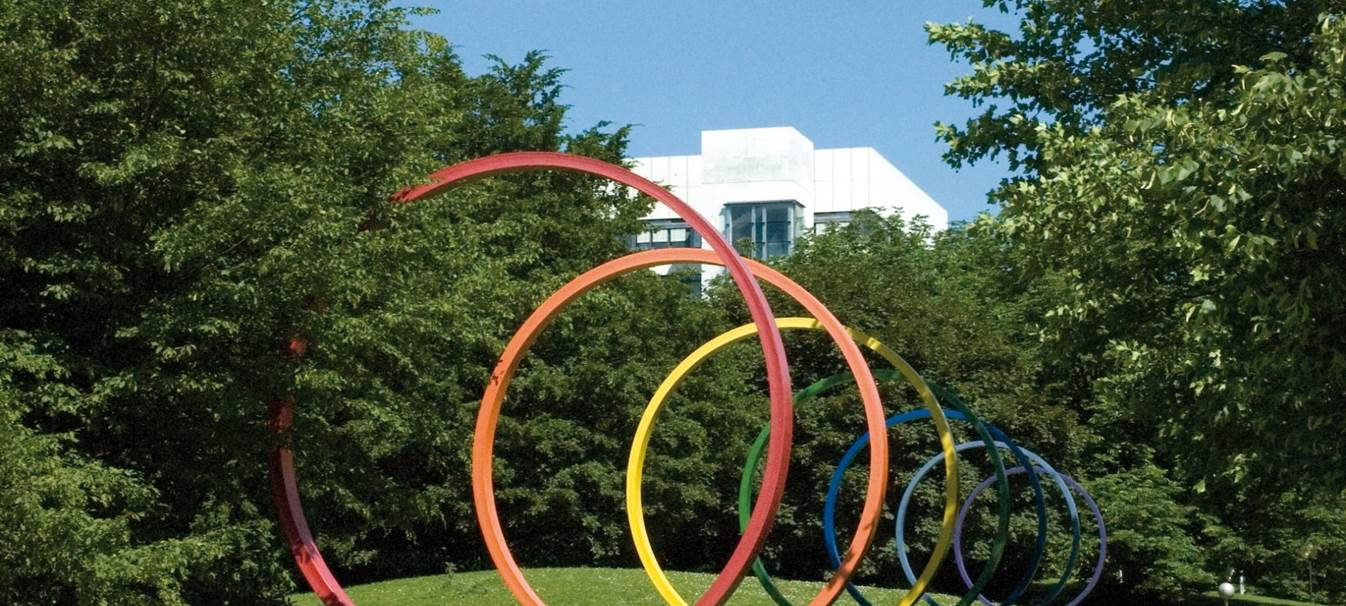
\includegraphics[width=\textwidth]{./TUDo-Title-Pic-2.jpg}
        \end{column}
    \end{columns}
\end{frame}

\begin{frame}
    \frametitle{Zwei Spalten für Text/Bild}
    % Für Bilder Argument T benutzen:
    \begin{columns}[T]
        \begin{column}{0.49\textwidth}
					\centerline{\textit{\small Feld links oben}}
        \end{column}
        \begin{column}{0.49\textwidth}
					\centerline{\textit{\small Feld rechts oben}}
				  \centerline{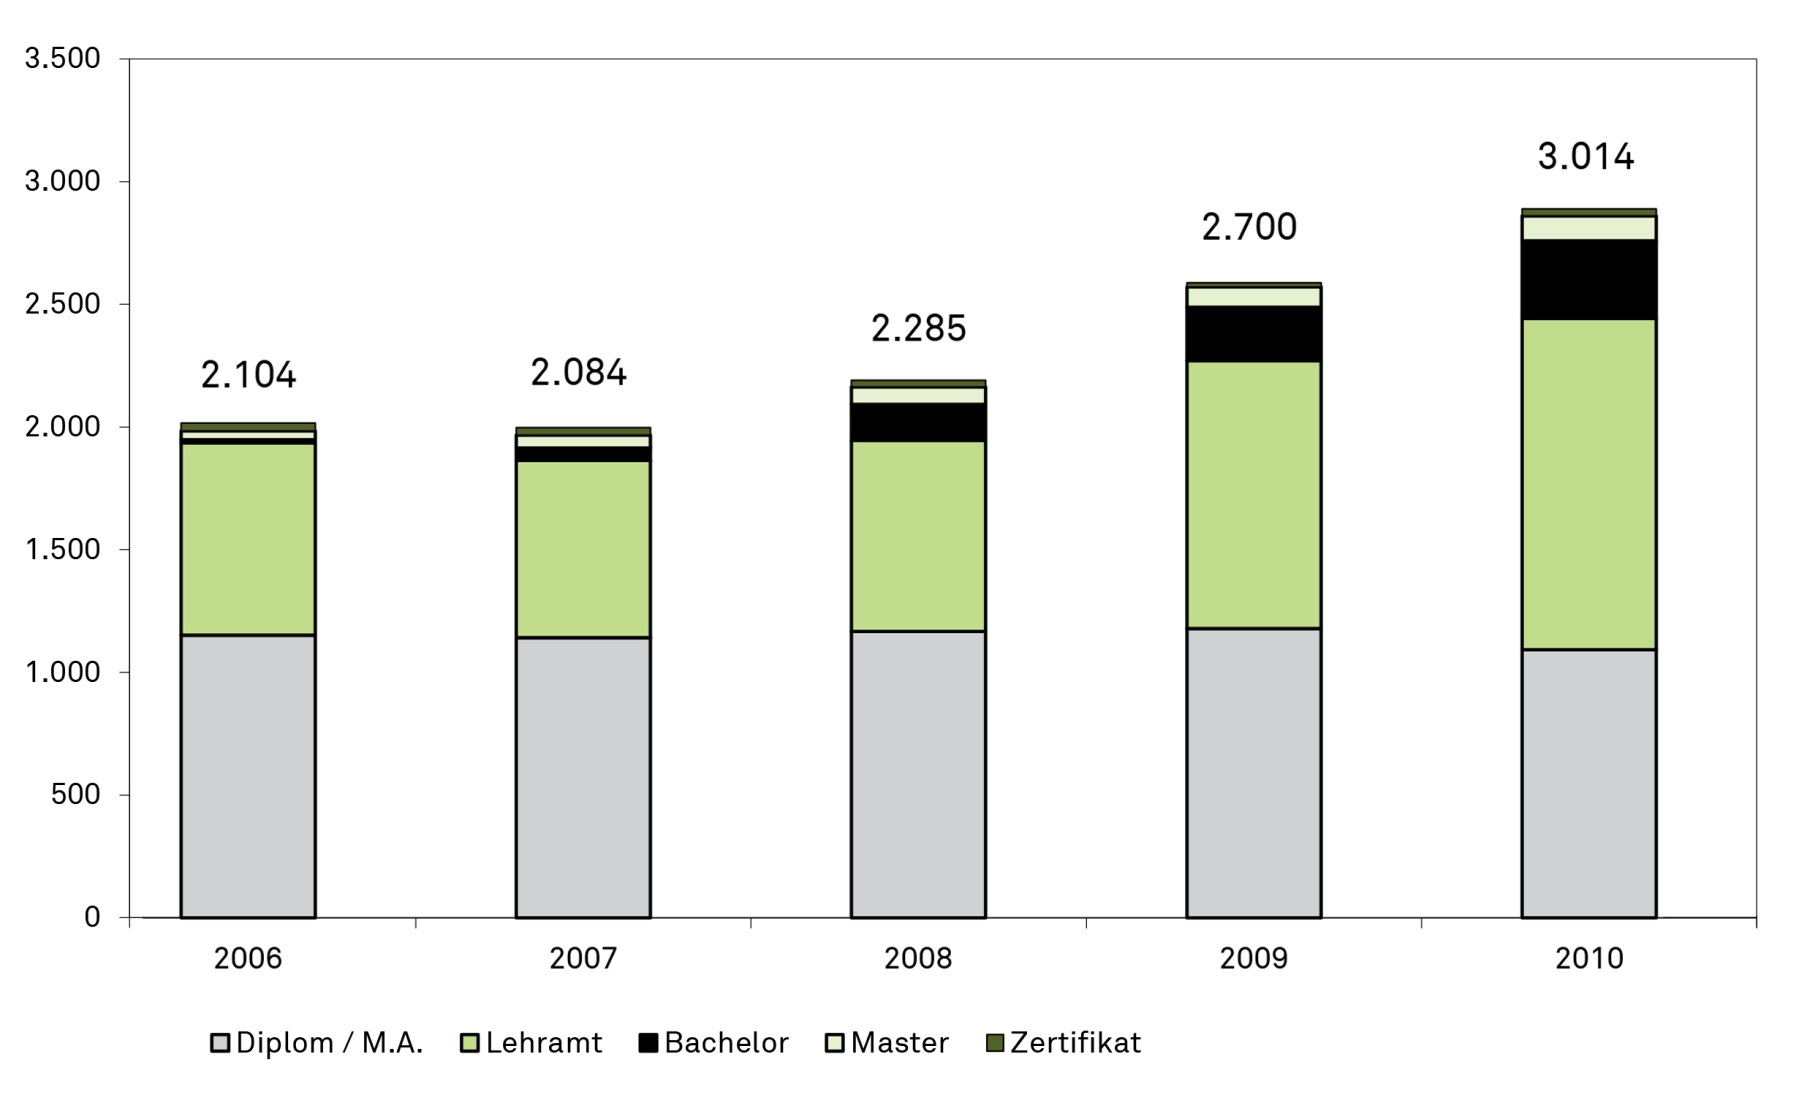
\includegraphics[width=0.75\textwidth]{./Pic-01.jpg}}
        \end{column}
    \end{columns}
    \medskip
    \begin{columns}[b]
      \begin{column}{0.49\textwidth}
				\centerline{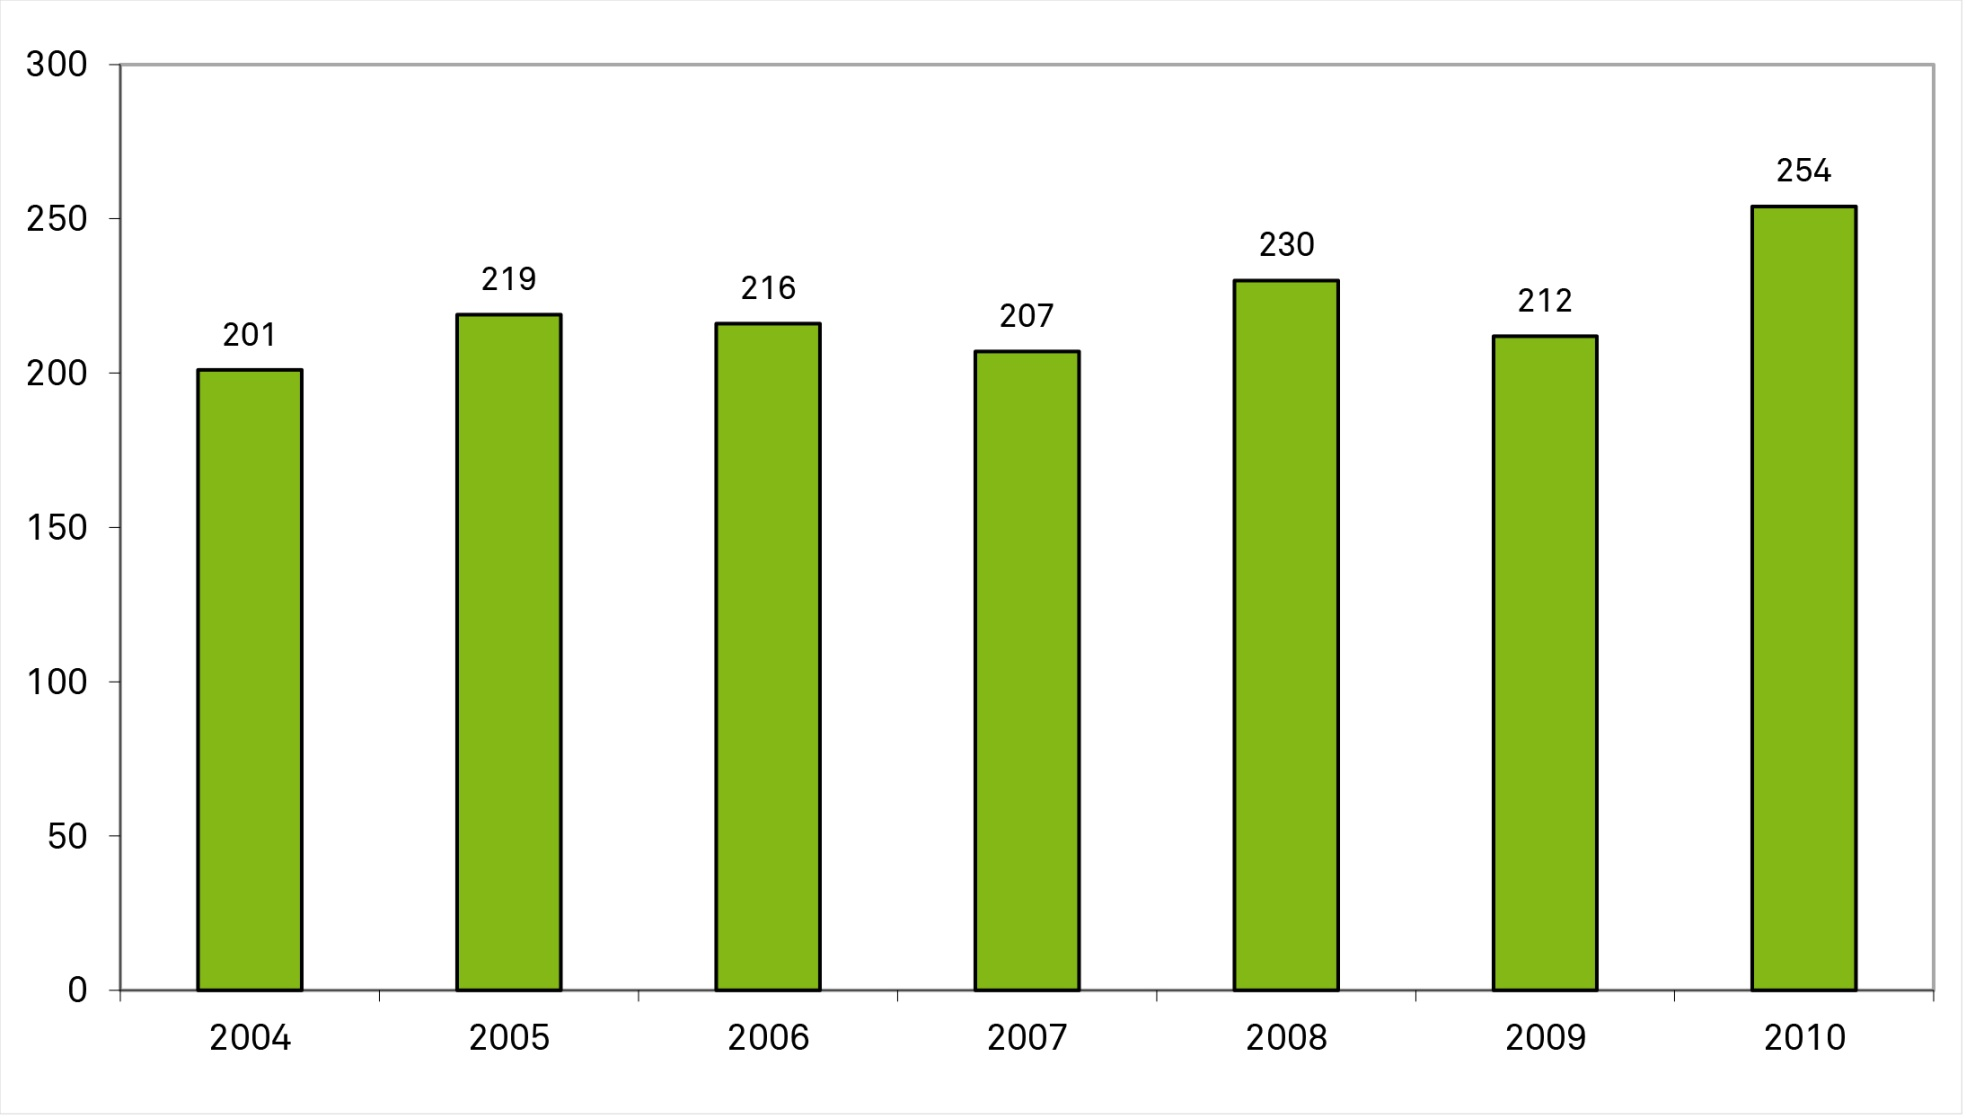
\includegraphics[width=0.75\textwidth]{./Pic-02.jpg}}
				\centerline{\textit{\small Feld links unten}}
			\end{column}
      \begin{column}{0.49\textwidth}
				\centerline{\textit{\small Feld rechts unten}}
      \end{column}
    \end{columns}
\end{frame}
\end{document}
